\chapter{Solução Proposta}
\label{cap:solucao}

O CHOReOS \ee (EE) é um middleware implementado no contexto deste trabalho.
Uma vez instanciado, ele fornece serviços que automatizam
a implantação de composições de serviços em ambientes de computação em nuvem,
funcionando no modelo de computação em nuvem denominado Plataforma como um Serviço (PaaS).

Para utilizar o EE, o usuário (implantador) deve descrever a composição a ser implantada
na Linguagem de Descrição Arquitetural do EE, uma especificação de alto nível que
diz \emph{o que} deve ser implantado, e não o \emph{como}. 
Finalmente, o usuário deve fornecer essa descrição ao EE através de sua API remota.

As funcionalidades fornecidas pelo \ee ao usuário são as seguintes:

\begin{itemize}
\item Criação automatiza de infraestrutura virtualizada (nós na nuvem).
\item API para automatizar a implantação de coreografias na nuvem.
\item Implantação escalável de coreografias de grande escala.
\item Suporte a implantação multi-nuvem.
\item Utilização de serviços de terceiros na composição a ser implantada.
\item Implantação automatizada de infraestrutura de monitoramento dos recursos utilizados.
\item Deleção automática de recursos da nuvem não utilizados.
\item API para escalamento vertical e horizontal.
\end{itemize}

Para a implementação do arcabouço Enactment Engine contribuíram Daniel Cuckier, Carlos Eduardo do Santos, Felipe Pontes, Alfonso Diaz, Nelson Lago, Paulo Moura, Thiago Furtado e demais colegas dos projetos Baile e CHOReOS. O \ee é software livre 
sob a Licença Pública da Mozilla 2\footnote{\url{http://www.mozilla.org/MPL/2.0/}} 
e está disponível em \url{http://ccsl.ime.usp.br/enactmentengine}. 

Neste capítulo, nós apresentamos a arquitetura e aspectos de implementação do \ee.   
Destacamos ao final do capítulo
como as decisões arquiteturais e de implementação auxiliam o implantador
a superar os desafios presentes na implantação de coreografia de grande escala.
Alguns aspectos aqui discutidos serão o tratados em alto nível,
priorizando o que é importante para o entendimento das contribuições
acadêmicas deste trabalho.
Detalhes de mais baixo nível sobre nosso middleware, principalmente do ponto de vista do
usuário, podem ser encontrados no \userguide.

Conforme já anunciado no Capítulo~\ref{cap:implantacao},
lembramos que para as descrições que se seguem utilizaremos
termos técnicos como definidos no DEPL~\cite{DEPL2006}.

\section{Arquitetura}

A arquitetura do \ee é exibida na Figura~\ref{fig:arquitetura}.

\begin{figure}[ht]
\centering
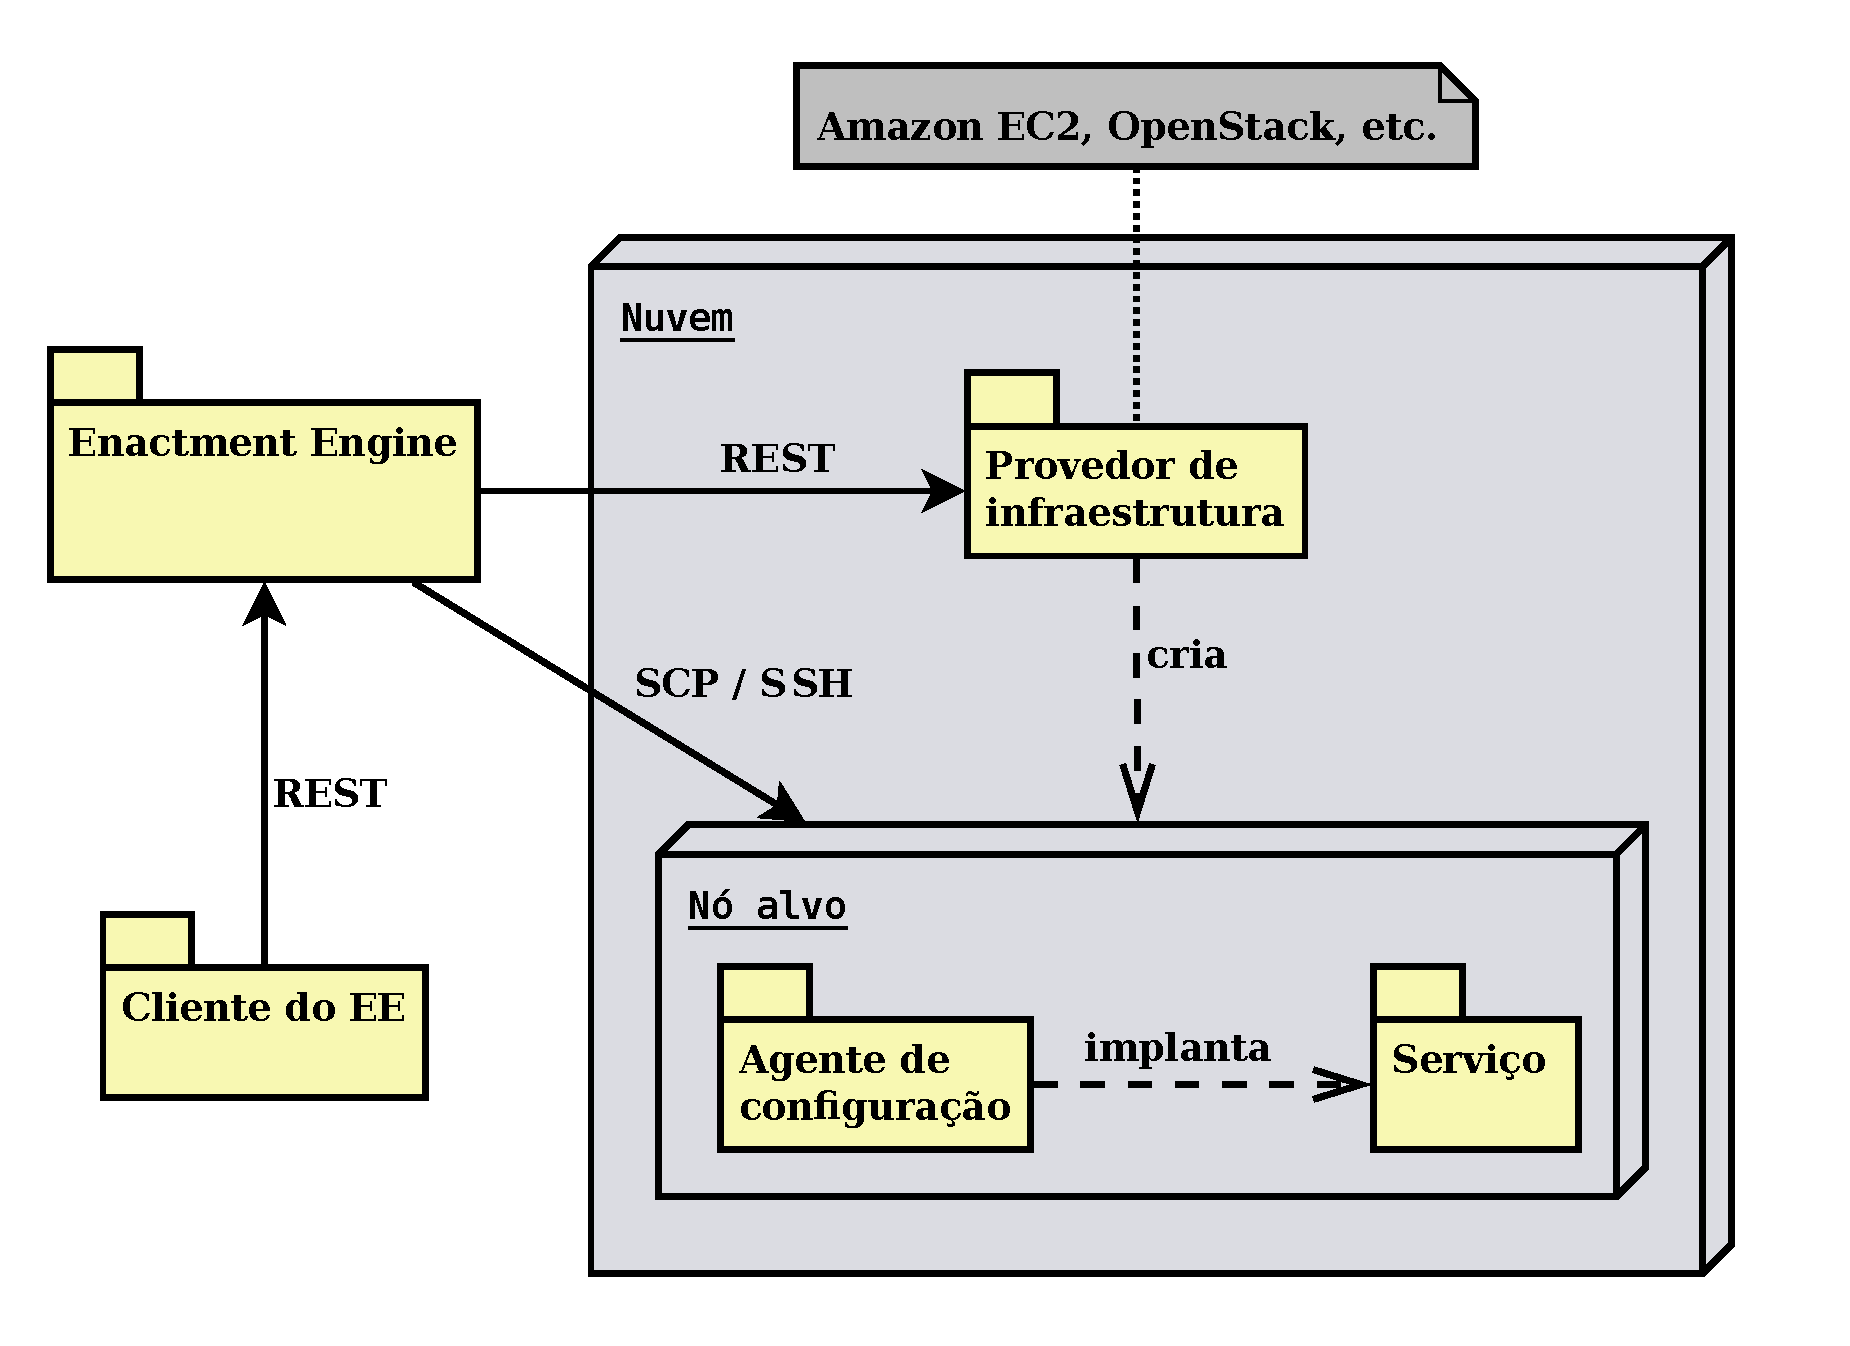
\includegraphics[width=0.7\linewidth]{arquitetura.pdf}
\caption{Arquitetura do \choreos \ee.}
\label{fig:arquitetura}
\end{figure}

\begin{itemize}

\item O \emph{Cloud Gateway} é um serviço de terceiros capaz de criar e destruir máquinas virtuais 
(também chamadas de \emph{nós}), normalmente em um ambiente de computação em nuvem. 
Atualmente o \ee suporta o Amazon EC2 e o OpenStack.

\item O \emph{agente de configuração} é executado nos nós alvos
e dispara os scripts que implementam as fases de preparação
e inicialização da implantação dos serviços.
O \ee utiliza o Chef Solo\footnote{\url{http://docs.opscode.com/chef_solo.html}}
como seu agente de configuração.

\item O \emph{cliente do \ee} é um programa ou script desenvolvido
pelo implantador, onde a especificação da coreografia é definida.
Esse script deve enviar a especificação da coreografia para o \ee
através das operações REST fornecidas pelo \ee.
Uma opção para implementar essas chamadas é utilizar
a biblioteca Java por nós fornecidas, que abstrai os detalhes
das chamadas REST.

\item O \emph{\ee} implanta os serviços da coreografia
com base na especificação enviada pelo cliente.
O processo implementado pelo \ee para efetuar a implementação
é descrito na Figura~\ref{fig:processo}, e explicado logo em seguida. 
\todo{explicar q é um serviço, mas q deve ser instalado}

\end{itemize} 

A Figura~\ref{fig:processo} exibe o processo de implantação de composições
de serviços implementado pelo \ee:

\begin{figure}[ht]
\centering
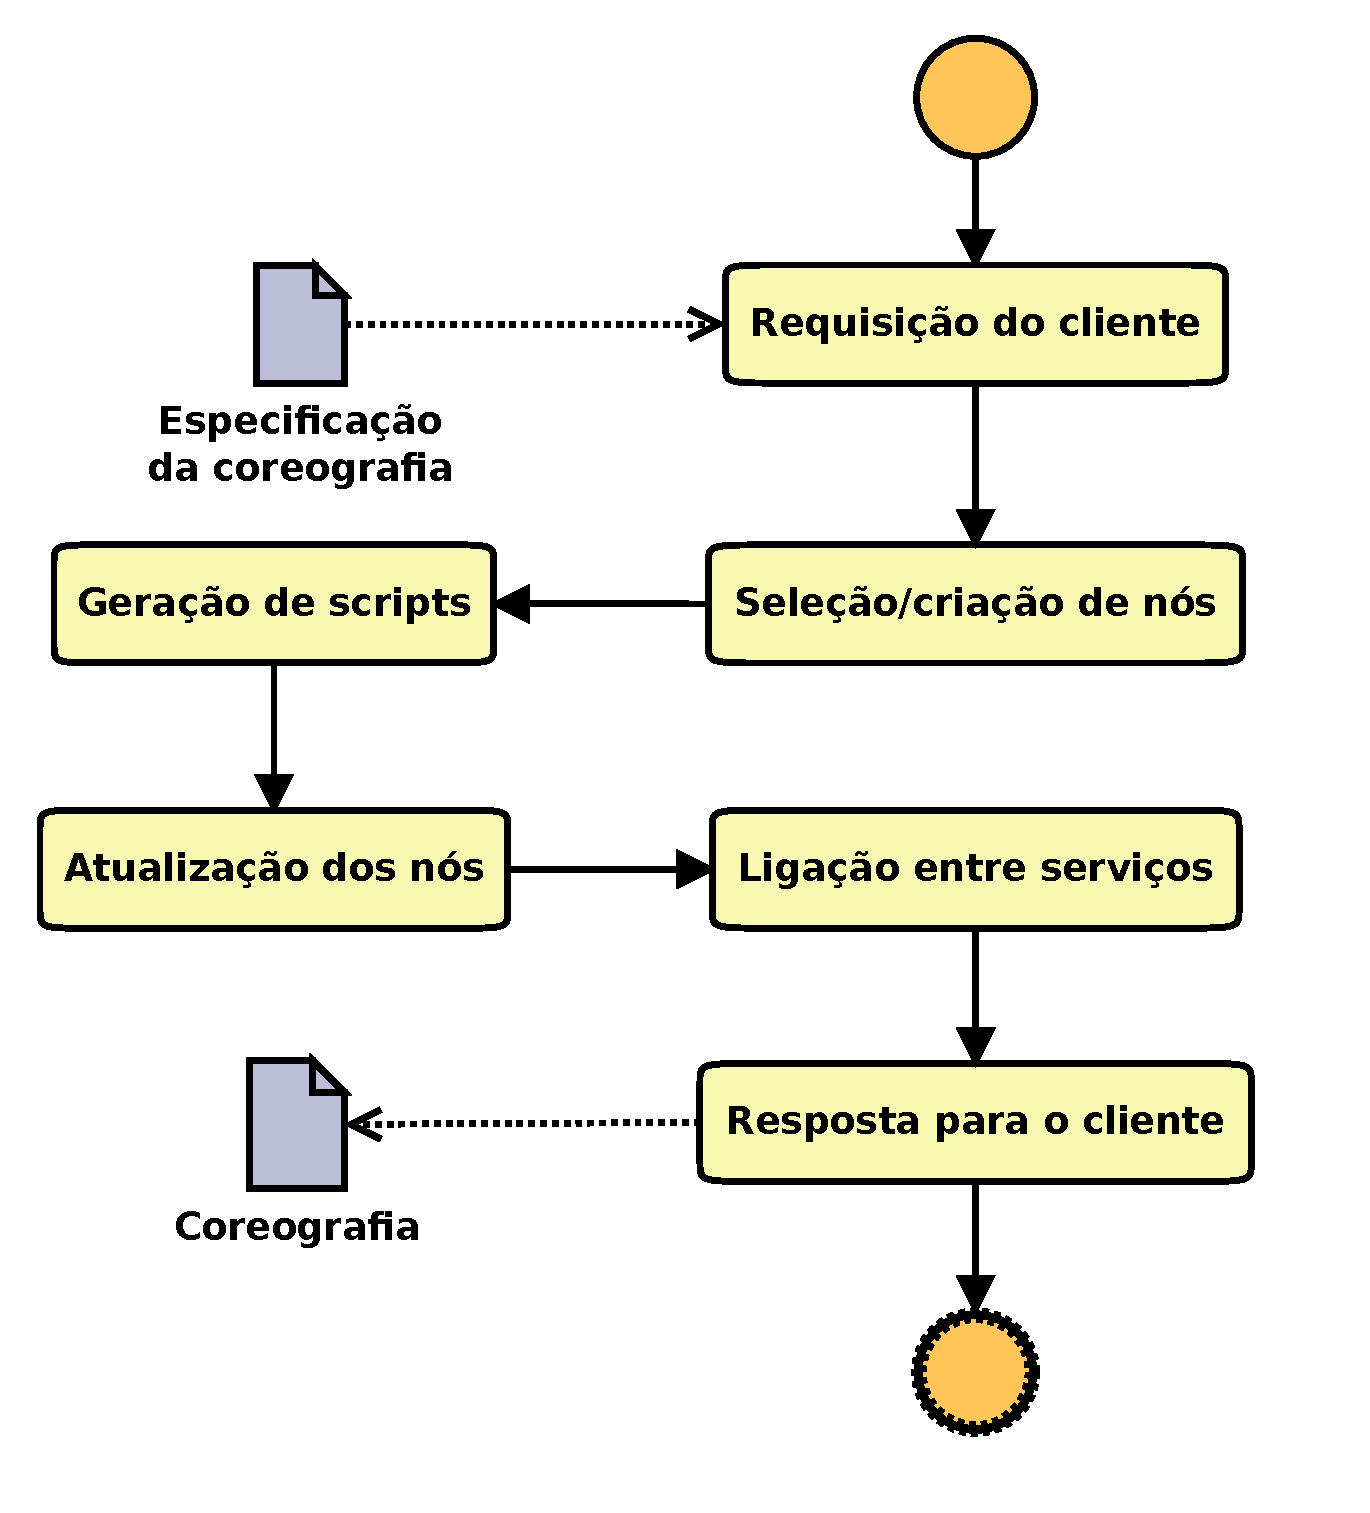
\includegraphics[width=0.5\textwidth]{processo.pdf}
\caption{Processo de implantação implementado pelo \ee.}
\label{fig:processo}
\end{figure}

\begin{enumerate}

\item \emph{Requisição do cliente:} o EE recebe a especificação da coreografia a ser implantada.
O formato dessa especificação é descrito na Seção~\ref{sec:spec}.

\item \emph{Seleção/criação de nós}: para cada serviço especificado, o EE seleciona um ou mais nós 
onde o serviço será implantado (um serviço pode ter várias réplicas implantadas). 
Se preciso, o EE requisitará ao Cloud Gateway a criação de novos nós.
Esse processo de seleção/criação de nós pode levar em conta os requisitos não-funcionais
dos serviços a serem implantados.
A política de seleção de nós é extensível, sendo definida pela organização
gerenciadora da instância do EE em execução. Algumas políticas já fornecidas são
``sempre cria um novo nó'' e ``cria novos nós até um certo limite, depois faz rodízio entre eles''.
Mais informações sobre a extensibilidade da política de seleção
são fornecidas na Seção~\ref{sec:extensao}.

\item \emph{Geração de scripts}: para cada serviço da coreografia, o EE gera dinamicamente os scripts de configuração do ambiente e inicialização do serviço. 
O EE configura então o agente de configuração do nó alvo para aquele serviço 
para que o script seja executado.

\item \emph{Atualização dos nós}: para cada nó alvo que receberá serviços da coreografia,
o EE dispara a execução do agente de configuração, de forma que o serviço é efeticamente
implantado e inicializado no nó.

\item \emph{Ligação entre serviços}: após os serviços terem sido iniciados, 
para cada relação de dependência na coreografia (ex: serviço \textsf{TravelAgency}
depende do serviço \textsf{Airline}), o EE fornece o endereço da dependência 
(ex: \url{http://airline.com/ws}) ao serviço dependente.
Mais informações sobre o processo de ligação são fornecidas na Seção~\ref{sec:ligacao}.
A implementação padrão para efetivar a ligação entre serviços, é a invocação de uma
operação SOAP, denominada \texttt{setInvocationAddress} no serviço dependente. 
Esse comportamento padrão pode ser modificado por extensão do EE,
conforme explicado adiante na Seção~\ref{sec:extensao}.

\item \emph{Resposta para o cliente}: o EE responde ao seu cliente,
fornecendo informações sobre em que nó cada serviço foi implantado,
e as URIs de acesso a cada serviço da coreografia.
O formato da resposta é descrito na Seção~\ref{sec:spec}.

\end{enumerate}

Há também alguns outros passos opcionais que não são aqui descrito por estarem fora
do escopo deste trabalho. Um exemplo é a implantação da infra-estrutura de monitoramento
dos nós alvos. O agente de monitoramento 
(Ganglia\footnote{\url{http://ganglia.sourceforge.net}})
é implantado nos nós alvos pelo EE e
coleta valores de uso de CPU, memória e disco dos nós.
\todo{para onde isso é enviado?}

\section{Especificação da coreografia}
\label{sec:spec}

O Enactment Engine recebe de seus clientes a especificação da coreografia na forma 
de uma descrição arquitetural com as informações necessárias e suficientes para 
que se possa realizar a implantação da coreografia. 
O Enactment Engine também devolve ao seu cliente informações sobre a implantação da coreografia, 
em especial as localizações de acesso aos serviços. As descrições da coreografia e de sua 
especificação são feitas com uma Linguagens de Descrição Arquitetural, assim como a dos trabalhos vistos no Capítulo~\ref{cap:relacionados}. 
A nossa ADL consiste na descrição de objetos relacionados entre si seguindo 
a estrutura de classes apresentada na Figura~\ref{fig:adl}. 
Em nossa implementação, essa descrição é realizada com representações em XML, 
que são trocadas entre o Enactment Engine e seu cliente. 
A descrição detalhada de cada atributo e o \emph{schema} XML da linguagem
são apresentados no \userguide.

\begin{figure}[!h]
  \centering
  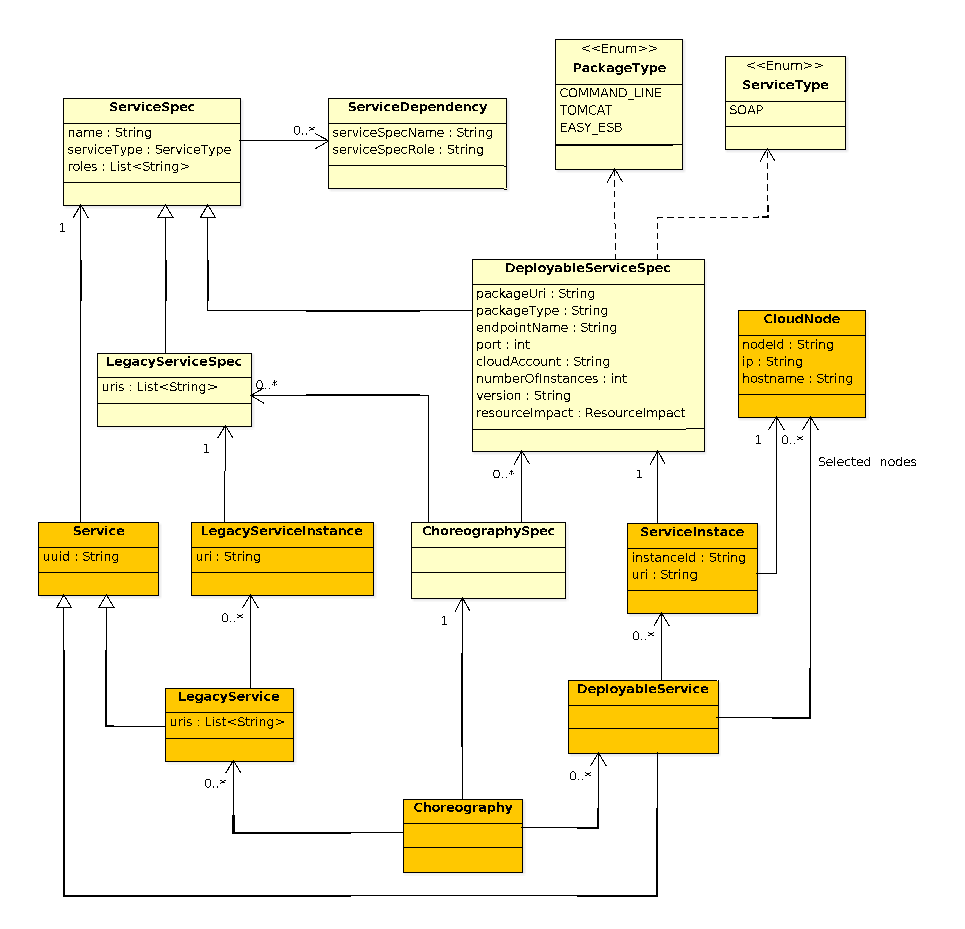
\includegraphics[width=.90\textwidth]{adl.pdf} 
  \caption{Estrutura da descrição arquitetural de uma coreografia}
  \label{fig:adl} 
\end{figure}

\todo{destacar q a chor spec mostra oq, e não o como}

A especificação da coreografia fornece todas as informações para a implantação da composição.
Para cada serviço, especifica-se de onde o pacote do serviço pode ser baixado
e qual o tipo do pacote (WAR, JAR, etc.).
Pode-se também especificar também para a coreografia a existência de serviços
de terceiros que já estão disponíveis na Internet e que devem
ser consumidos por serviços da coreografia.
O implantador pode escrever a especificação da coreografia diretamente em XML
ou utilizar objetos Java (POJOs).
A Listagem~\ref{lst:service_spec} apresenta um trecho da especificação de uma coreografia,
no qual um dos serviços participantes é definido,
incluindo sua dependência de outro serviço da coreografia.

\lstset{
language=Java,
}

{\scriptsize
\begin{lstlisting}[breaklines, caption={Trecho da especificação de uma coreografia.}, label={lst:service_spec}]
airportBusCompanySpec =
  new DeployableServiceSpec(AIRPORT_BUS_COMPANY, ServiceType.SOAP, PackageType.COMMAND_LINE, resourceImpact, serviceVersion, AIRPORT_BUS_COMPANY_JAR_URL, AIRPORT_BUS_COMPANY_PORT, AIRPORT_BUS_COMPANY, numberOfReplicas);
airportBusCompanySpec.setRoles(
  Collections.singletonList(AIRPORT_BUS_COMPANY));
airportBusCompanySpec.addDependency(
  new ServiceDependency(AIRPORT_name, AIRPORT_endpoint));
\end{lstlisting}
}

\section{Ligação entre serviços}
\label{sec:ligacao}

Segundo Dearle~\cite{Dearle2007PastPresentFuture}, componentes podem ser ligados entre si em vários momentos: compilação, montagem, configuração e execução. Em nosso contexto, a ligação deve ser efetuada necessariamente em tempo de execução, pois é somente nesse momento que teremos os endereços completos dos serviços implantados. Uma das possibilidades apontadas por Dearle para efetivação da ligação em tempo de execução é a utilização do padrão de injeção de dependência, conforme introduzido por Fowler~\cite{Fowler2004Inversion}. A injeção de dependências é utilizada em contêineres como o Springer\footnote{\url{http://www.springer.org}}, no qual o middleware passa ao componente referências de suas dependências. No entanto, Dearle ainda alega que há uma falta de arcabouços para a aplicação da injeção de dependência de forma distribuída.

A solução adotada no \ee\ para possibilitar a ligação entre serviços envolve a utilização do middleware para a passagem de endereços dos serviços implantados aos seus consumidores, o que é feito com base na lista de objetos \textsf{ServiceDependency} pertencentes a um \textsf{ChorServiceSpec}. Essa solução consiste na aplicação do padrão de injeção de dependência de forma distribuída, e é similar ao que foi feito nos trabalhos sobre a linguagem Darwin~\cite{Magee1996Dynamic, Magee1994Regis}. Para que esse processo funcione, é preciso que cada serviço na coreografia que possua dependências implemente uma operação denominada \texttt{setInvocationAddress}, por nós padronizada. Essa operação recebe como argumentos as seguintes informações sobre a dependência: papel do serviço, nome do serviço no contexto da coreografia e as URIs de acesso ao serviço.  Em uma coreografia em que, por exemplo, um serviço de agência de viagem dependa do serviço de uma companhia aérea, o \ee\ poderá executar a seguinte invocação ao serviço da agência de viagens : \texttt{setInvocationAddress('Companhia Aérea', 'Nimbus Airline', [ 'http://192.168.56.107:8080/nimbus/ws/' ])}. Nessa solução, a ``inteligência'' em determinar quais serviços satisfazem as necessidades de outros serviços está na camada que produz a entrada do \ee.

\todo{descrever primeiro genericamente, e depois com o setInvocationAddress,
que é apenas uma possível implementação}.

\todo{explicar para que serve o nome do serviço}/

Apesar dos benefícios de uma solução como essa, Dearle~\cite{Dearle2007PastPresentFuture} também alerta sobre a desvantagem em forçar componentes a aderirem convenções de codificação impostas pelo middleware, o que poderia restringir o serviço a uma determinada linguagem de programação ou a algum middleware específico. Reconhecemos que esse problema existe em nossa solução, mas acreditamos que o desenho adotado ameniza os problemas levantados, pois tudo o que o serviço é obrigado a fazer é implementar a operação \texttt{setInvocationAddress} e conhecer os papeis de suas dependências, o que implica em conhecer a interface sintática de cada papel. Dessa forma, nossa solução não restringe o serviço a nenhuma linguagem e possibilita seu uso por outros middlewares que adotem a mesma convenção para o \texttt{setInvocationAddress}.

\section{Interface do \ee}
\label{sec:interface}

Os clientes do \ee utilizam suas funcionalidades por meio de uma API REST, que é descrita nesta seção. 
Por se tratar de uma API REST, o cliente pode ser implementado em qualquer linguagem 
e ambiente que possua alguma biblioteca HTTP. 
Também disponibilizamos um cliente na forma de uma biblioteca na linguagem Java, 
tornando o uso do \ee ainda mais simples para os usuários da linguagem Java, 
atualmente uma das mais utilizadas do mercado. 
Seguimos agora com uma descrição de alto nível de cada uma das operações disponíveis 
na API REST do \ee. Detalhes da API, como os códigos de status HTTP retornados, 
são fornecidos no \userguide.

\begin{description}

\item [Criar coreografia:] registra a especificação de uma coreografia no \ee. 
Essa especificação é a descrição arquitetural da coreografia, 
estruturada de acordo com a classe \textsf{ChorSpec} (ver Seção~\ref{sec:spec}). 
Essa operação não realiza a implantação da coreografia.

\item [Obter coreografia:] obtém informações sobre uma coreografia registrada no \ee. 
Essas informações referem-se à especificação da coreografia e ao estado da implantação 
de seus serviços, como os nós em que os serviços foram implantados, 
no caso de a implantação já ter sido realizada.

\item [Encenar coreografia:] realiza a implantação de uma coreografia já registrada no \ee. 
Ao fim do processo, detalhes do resultado da implantação são retornados na representação XML da coreografia. 
A implementação dessa operação deve possuir duas importantes propriedades: 
1) a falha na encenação de parte da coreografia não deve interromper a encenação do resto da coreografia; 
2) a operação deve ser \emph{idempotente}, ou seja, uma nova requisição para a encenação da mesma 
coreografia não deve tentar implantar os serviços já implantados, 
mas somente aqueles cujas implantações falharam na última execução. 
Para que serviços sejam atualizados, é preciso utilizar um novo valor no atributo ``versão'' da especificação do serviço.

\item [Atualizar coreografia:] registra uma nova versão de uma coreografia no \ee. 
Os serviços atualizados na nova versão da coreografia devem possuir 
um novo número de versão em suas especificações. 
Essa operação, assim como a criação da coreografia, não encena a nova coreografia. 
Para isso, é preciso invocar novamente a operação de encenação.

A atualização de serviços não é o foco de nosso trabalho.
Dessa forma, em nosso trabalho a atualização dos serviços será feita da forma mais simples possível: 
apenas substituindo o serviço existente por sua nova versão. 
Contudo, tal procedimento pode provocar falhas na comunicação entre os serviços de uma coreografia. 
Vários trabalhos \cite{Kramer1990Philosophers, Vandewoude2007Tranquility, Xiaoxing2011VersionConsistent} 
estudam o processo de atualização dinâmica, pelo qual as conversações correntes 
são preservadas durante a atualização de um serviço. 
Embora não esteja no escopo de nosso trabalho, esperamos que a arquitetura do \ee possa ser 
evoluída para que a operação de atualização de coreografia utilize procedimentos seguros de 
atualização dinâmica, dentre os quais destacamos a proposta de Xiaoxing et al~\cite{Xiaoxing2011VersionConsistent}.

\end{description}

Na Listagem~\ref{lst:java_chor_enactment} fornecemos um exemplo de como seria
um programa Java invocando o \ee para implantar uma coreografia.
Nesse exemplo, a classe \textsf{MyChorSpec} está escondendo a declaração
da especificação da coreografia.

\begin{lstlisting}[breaklines, caption={Programa Java que invoca o \ee para implantar uma coreografia.}, label={lst:java_chor_enactment}]
public class Enactment {

    public static void main(String[] args) throws EnactmentException, ChoreographyNotFoundException {

        final String EE_URI = "http://localhost:9102/enactmentengine";
        EnactmentEngine ee = new EnactmentEngineClient(EE_URI);
        ChoreographySpec chorSpec = MyChorSpec.getChorSpec();

        String chorId = ee.createChoreography(chorSpec);
        Choreography chor = ee.enactChoreography(chorId);

        System.out.println(chor); // vamos ver o que aconteceu...
    }
}
\end{lstlisting}


\section{Pontos de extensão}
\label{sec:extensao}

Para lidar com as particularidades do ambiente de cada organização, o Enactment Engine fornece alguns pontos de extensão. Esses pontos de extensão são classes que desenvolvedores devem escrever na linguagem Java e que, de acordo com as configurações do sistema, poderão ser executadas pelo arcabouço.
Neste capítulo descreveremos os pontos de extensão de nosso middleware, 
mostrando as interface associadas a cada um deles.
Para mais detalhes sobre todos os passos necessários para implementar
uma extensão, verificar o \userguide.

\begin{description}

\item [Infraestrutura de nuvem:] implementando a interface \textsf{CloudProvider} é possível o suporte a novas plataforma de computação em nuvem. Atualmente nossa implementação suporta o serviço EC2 do AWS e o OpenStack.

\begin{lstlisting}[frame=trbl, label=lst:cloud_provider, caption=Interface CloudProvider.]
/**
 * Provides access to cloud service functions to create nodes on the cloud.
 * 
 * Each specific provider (e.g. AmazonWS) must have an implementing class 
 * of this interface.
 * 
 */
public interface CloudProvider {

    public String getCloudProviderName();

    public CloudNode createNode(NodeSpec nodeSpec) throws NodeNotCreatedException;

    public CloudNode getNode(String nodeId) throws NodeNotFoundException;

    public List<CloudNode> getNodes();

    public void destroyNode(String id) throws NodeNotDestroyed, NodeNotFoundException;

    public CloudNode createOrUseExistingNode(NodeSpec nodeSpec) throws NodeNotCreatedException;

    public void setCloudConfiguration(CloudConfiguration cloudConfiguration);

}
\end{lstlisting}

\todo{explicar cloud configuration?}

Para facilitar o desenvolvimento de novas implementações,
nós fornecemos uma implementação base, a classe \textsf{JCloudsCloudProvider}.
Ela utiliza a biblioteca JClouds\footnote{\url{http://jclouds.incubator.apache.org/}},
que já é apta a acessar uma ampla gama de provedores de infraestrutura disponíveis no mercado.
Essa implementação base foi utilizada para a implementação das classes 
\textsf{AmazonCloudProvider} e \textsf{OpenStackKeyStoneCloudProvider},
que contaram, respectivamente, com 79 e 96 linhas de código-fonte.

\todo{Classe base: JCloudsCloudProvider}

\item [Política de seleção de nós:] a implementação da interface \textsf{NodeSelector} define uma nova política de alocação de serviços em nós da nuvem, que pode levar em conta os requisitos não-funcionais do serviço e propriedades dos nós à disposição.
Algumas políticas já fornecidas são ``sempre cria um novo nó'' e 
``cria novos nós até um certo limite, depois faz rodízio entre eles''.

\begin{lstlisting}[frame=trbl, label=lst:node_selector, caption=Interface NodeSelector acompanhada de sua classe pai Selector.]
/**
 * Selects a node to apply a given configuration
 * 
 * The selection can consider functional requirements, which is provided by
 * spec.resourceImpact. Implementing classes must use the NodePoolManager 
 * to retrieve nodes AND/OR create new nodes. 
 * NodeSelectors are always accessed as singletons. 
 * Implementing classes must consider concurrent access to the
 * selectNodes method.
 *  
 */
public interface NodeSelector extends Selector<CloudNode, DeployableServiceSpec> {

}

/**
 * Selects objects from a given source according to the requirements. 
 * If necessary, creates new objects using a given factory.
 * 
 * 
 * @param <T>
 *            the class of the selected resource
 * @param <R>
 *            the class of the requirements
 */
public interface Selector<T, R> {

    public List<T> select(R requirements, int objectsQuantity) throws NotSelectedException;

}
\end{lstlisting}

Formas similares dessa funcionalidade são também utilizadas em estudos já apresentados na seção de trabalhos relacionados.  O trabalho de Magee e Kramer~\cite{Magee1997Corba} apresenta a seleção de nós em função da utilização de CPUs nos nós existentes, não havendo possibilidade de utilização de outros critérios, como memória, disco, custo etc. Nos sistemas apresentados por Dolstra et al.~\cite{Dolstra2005Configuration} e Balter et al.~\cite{Balter1998Olan} é preciso que a distribuição dos serviços seja especificada com o uso dos IPs das máquinas nas quais os serviços devem ser implantados, o que não é possível em um ambiente de nuvem. Por fim, o \emph{broker} apresentado por Watson et al. é o componente que mais se assemelha ao nosso NodeSelector, pois os autores deixam claro que várias implementações diferentes são possíveis, considerando-se diferentes tipo de requisitos e diferentes fontes de monitoramento. Como a escolha é feita em tempo de execução do serviço, seria também possível uma seleção que independa de IPs estabelecidos em tempo de projeto. No entanto, os autores não explicam como os usuários de seu sistema, os provedores de infraestrutura, deveriam proceder para criar seus próprios \emph{brokers} personalizados.

Para avançar em relação às limitações dos trabalhos anteriormente citados,  consideramos como requisitos principais a dinamicidade do ambiente de nuvem, que nos impede de conhecer os IPs das máquinas em tempo de configuração, bem como a flexibilidade para que cada organização determine os requisitos de distribuição dos serviços.

\item [Tipos de pacotes de serviços:] um serviço pode ser distribuído por diferentes tipos de pacotes, como em um JAR ou em um WAR, por exemplo. Como existem muitas outras opções, é preciso que esse seja um ponto de flexibilidade. Para cada novo tipo de pacote, pode-se escrever um template de um \emph{cookbook} Chef que implemente a preparação e a inicialização do serviço. \todo{falar mais dos tokens no template...}

\item \emph{Package type:} the current supported types
are JAR and WAR packages. Users may add support to a new package type
by writing a Chef cookbook template.
One example would be a Python web service deployment in an Nginx server.

\item [Tipos de serviços:] a ligação entre serviços de uma coreografia depende da passagem de endereços que é feita do \ee para os serviços. Para isso, o EE precisa invocar a operação \texttt{setInvocationAddres} dos serviços. A implementação de tal invocação dar-se-á de forma diferente se o serviço for SOAP ou REST. A implementação da interface \textsf{ContextSender} possibilita ao EE realizar a invocação da operação \texttt{setInovcationAddress} em serviços de outras tecnologias (JMS e CORBA por exemplo). Nota-se que para cada um desses tipos de serviços adicionados pelo usuário, é preciso criar uma convenção para a assinatura sintática da operação \texttt{setInvocationAddres}.

\begin{lstlisting}[frame=trbl, label=lst:context_sender, caption=Interface ContextSender.]
public interface ContextSender {

    /**
     * Calls setInvokationAddress operation on service 
     * in the serviceEndpoint.
     * So, the service in endpoint will know that its 
     * partner named partnerName with partnerRole is 
     * realized by instances in partnerEndpoints.
     * 
     * @param serviceEndpoint
     * @param partnerRole
     * @param partnerName
     * @param partnerEndpoints
     * @throws ContextNotSentException
     *             if context was not successfully set
     */
    public void sendContext(String serviceEndpoint, 
                            String partnerRole, 
                            String partnerName, 
                            List<String> partnerEndpoints) throws ContextNotSentException;
}
\end{lstlisting}

\end{description}


\section{Aspectos gerais de implementação}

\section{Aspectos da implementação que auxiliam na superação dos desafios de implantação de coreografias de grande escala}

\subsection{Confiança no processo de implantação}
\label{subsec:process}

Tornar a implantação de sistemas ``\emph{Internet-scale}'' processos totalmente automatizados
é necessário para que a implantação se torne testável, flexível e confiável~\cite{Hamilton2007InternetScale}.
Enquanto implantar sistemas distribuídos de grande escala se torna uma atividade
morosa e propensa a erros~\cite{Dolstra2005Configuration},
o processo de implantação deveria ser automatizado,
conforme já é reconhecido por praticantes~\cite{Humble2011Continuous}.

O \ee possibilita a automação do processo de implantação
graças a sua interface remota (REST), que recebe a especificação
da composição a ser implantada e devolve o resultado do processo.

O uso de uma especificação declarativa,
como já utilizado em outros trabalhos~\cite{Balter1998Olan,Magee1996Dynamic},
também facilita o desenvolvimento do script de implantação
para cada nova composição a ser implantada.
Sem isso, a implantação automatizada também é possível,
com o reuso entre scripts implantadores de diferentes composições
se torna mais complicado, o que aumenta o tempo de trabalho
para se produzir novos scripts.

A tendência atual na implantação de sistemas de grande escala é o uso
de recursos elásticos possibilitados pela computação em nuvem.
Recursos virtualizados fornecidos pela nuvem potencializam
a automação do processo de implantação~\cite{Humble2011Continuous}.
Uma vez que a criação de todo um novo ambiente pode ser automatizado
pelo provisionamento de máquinas virtuais, cada nova implantação
pode facilmente criar um ambiente limpo onde os sistemas implantados
serão executados.
Reproducibilidade e isolamento entre ambientes são facilitados
ao se evitar passos manuais no preparo do ambiente.

Por outro lado, a utilização dos recursos de nuvem também trazem alguns desafios,
uma vez que se faz necessário levar em contar a natureza dinâmica da nuvem~\cite{Amazon2012Practices}.
Diferentemente dos cenários estudados em trabalhos anteriores sobre
implantação de sistemas baseados em componentes~\cite{Balter1998Olan,Magee1996Dynamic},
os nós alvos são mais dinâmicos, não sendo possível conhecer os endereços IPs
desses nós quando se está escrevendo a especificação da composição a ser implantada.
A ligação entre serviços deve ser feita em tempo de execução (via \texttt{setInvocationAddress})
e a política de alocação de nós deve ser flexível, i.e.,
um serviço não deve ser alocado a um IP estático antes do tempo de implantação.
O \ee possibilita que políticas de alocação de nós personalizadas
escolham em tempo de execução em que nós um serviço deve ser implantado,
considerando inclusive requisitos não-funcionais do serviço.

\subsection{Tratando falhas de terceiros}
\label{sec:failures}

Sistemas distribuídos de grande escala devem esperar e tratar falhas
de componentes de terceiros~\cite{Hamilton2007InternetScale,Helland2009Quicksand,CarnegieMellon2006ULS}.
Mesmo se a chance de falhas de cada componente é pequena,
a grande quantidade de componentes e interações aumenta as chances de 
falhas em algum lugar do sistema~\cite{CarnegieMellon2006ULS}.

Um exemplo de falhas típica em um ambiente de nuvem envolve o provisionamento de VMs.
Quando um novo nó é requisitado para o provedor de infraestrutura,
há uma chance de que o provisionamento irá falhar.
Além disso, alguns nós podem levar um tempo muito maior que a média para ficarem prontos.
Outras operações que podem falhar durante o processo de implantação são
conexões SSH e a execução de scripts nos nós alvos.

A Figura~\ref{fig:ec2_boxplot} mostra a distribuição observada
do tempo de criação de VMs quando se requisita concorrentemente a criação
de 100 nós na nuvem da Amazon (isso foi repetido 10 vezes).
Nós contamos o tempo que vai da requisição de criação do nó
até o momento em que a VM se encontra apta a receber conexões SSH,
que é quando ela se torna pronta para uso na prática.
Nós observamos uma taxa de falha de 0.6\%
quando se tenta criar concorrentemente 100 nós.
É interessante notar que o tempo de criação tem uma mediana estável,
mas que alguns valores altos para esse tempo são esperados quando
se cria ao mesmo tempo uma grande quantidade de nós.
Em nossas observações, falhas e tempos longos de provisionamento
afetaram até 7\% das requisições de criação de nós.

\begin{figure}[ht]
\centering
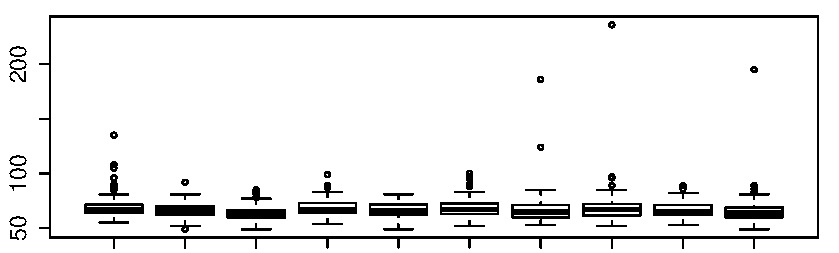
\includegraphics[width=\linewidth]{ec2_boxplot.pdf}
\caption{Tempos de criação de instâncias EC2 observados, em segundos.}
\label{fig:ec2_boxplot}
\end{figure}

\todo{o q tá até aqui é problema, mover pra outro lugar... 
daqui pra baixo é solução, q é oq deve estar aqui}

Uma abordagem simples adotada pelo \ee para tratar falhas externas
foi encapsular a lógica de invocação de sistemas externos em uma classe, 
chamada \textsf{Invoker}, e usá-la de uma forma disciplinada pelo projeto.
Nosso \textsf{Invoker} recebe os seguintes parâmetros:
uma \emph{tarefa}, que é uma rotina que se comunicará com algum sistema externo,
a quantidade de \emph{tentativas} para executar a tarefa,
o \emph{timeout} de cada tentativa, e um \emph{intervalo} entre as tentativas.

Uma instância do \textsf{Invoker} deve ser configurada deve ser configurada
de acordo com sua tarefa (por exemplo, nós descobrimos que três tentativas
não é o suficiente para transferência de arquivos por SCP).
Em vez de ter esses valores fixados no código-fonte, eles são explicitamente
ajustados em arquivos de configuração.
Desta forma, pode-se facilmente ajustar esses valores de acordo com 
as características do ambiente alvo.
Portanto, essa abordagem é também uma estratégia para colaborar 
com a heterogeneidade de plataformas e tecnologias.
A classe \textsf{Invoker} pode ser facilmente decorada\footnote{Ver padrão de projeto \emph{decorator}} para adaptar valores de timeouts automaticamente
baseando-se em heurísticas definidas programaticamente por engenheiros 
da comunidade DevOps.

O \ee adota uma estratégia particular par lidar com falhas durante a criação de novas VMs.
Quando uma requisição chega, o \ee tenta criar um novo nó.
Se a criação falha ou demora muito, um nó já criado é recuperado de uma reserva de nós ociosos.
Essa estratégia evita que se tenha que esperar novamente pelo tempo de se criar um novo nó.
A capacidade inicial da reserva é definida por configuração
e ela é preenchida cada vez que a criação de um nó é requisitada.
Se o tamanho da reserva é reduzido e alcança um dado limite,
a capacidade é aumentada, de forma a tentar evitar uma situação futura
de se encontrar uma reserva vazia em um momento de necessidade.

A abordagem da reserva impõe um custo extra de se manter algumas VMs a mais
em execução (em um estado ocioso). Contudo, esse problema é tratado
pelo \ee por um algoritmo de gerenciamento distribuído em cada nó:
se o nó está em um estado ocioso por $N-1$ minutos, onde $N$ é um limite
de tempo que implica custo adicional, o nó envia ao \ee um pedido para 
sua própria destruição. Assim, depois de um tempo de inatividade no \ee,
a reserva se torna vazia em algum momento, sendo preenchida novamente
somente quando chegam novas requisições de criação de nós.
%This distributed approach alleviates the need to have the \ee periodically check
%the status of the machines to decide whether they should be removed.

\todo{na amazon vc não é cobrado por instâncias paradas!}

Outra prática importante relacionada a tolerância a falhas é a 
\emph{degradação suave}~\cite{Brewer2001GiantScale,Hamilton2007InternetScale}.
Em nosso contexto, degradação suave significa que se um serviço não foi 
implantado apropriadamente, não é aceitável que o processo de implantação
de toda a composição seja interrompido.
Com o \ee, se algum serviço não é implantado, o processo de implantação continua,
e a resposta do \ee fornece informações sobre os problemas ocorridos,
possibilitando ações de recuperação.

Contudo, é importante destacar que a responsabilidade pela degradação suave
debe ser compartilhada com a implementação dos serviços, uma vez que cada serviço
debe saber como se comportar na ausência de uma ou mais de suas dependências.
De outra forma, cada serviço se tornaria um \emph{ponto de falha único} na composição,
o que é altamente indesejável.

\subsection{Escalabilidade}

Quando se implanta uma grande quantidade de serviços em um ambiente distribuído,
não é desejável que as implantações dos diferentes serviços sejam sequenciais.
Uma vez que a implantação de diferentes serviços são tarefas independentes,
implanta-los concorrentemente aumenta drasticamente a escalabilidade
do processo de implantação da composição.

Dizemos que uma arquitetura é perfeitamente escalável
se ela continua a apresentar o mesmo desempenho por recurso,
mesmo que usado em um problema de tamanho maior, conforme o número
de recursos aumenta~\cite{Quinn1994Scalability}.
No contexto de implantação, isso significa que, idealmente,
o tempo de implantação deveria permanecer constante quando há um
aumento proporcional no número de serviços a serem implantados e
no número de nós alvos.

Note que o número de serviços a ser implantado aumenta em duas situações:
1) quando se implanta composições maiores e 2) quando se implanta
mais composições simultaneamente. A segunda situação pode ocorrer, por exemplo,
quando se executa uma bateria de testes de aceitação de uma composição de serviços.
Em tal situação, é desejável que testes de aceitação sejam executados em paralelo,
o que requer implantação concorrente de múltiplas instâncias da mesma composição.
\todo{obs: testes de aceitação tendem a ser demorados; ex: engloba criação de VM.}

Embora o conhecimento de programação concorrente para implementar
um processo de implantação escalável seja básico (dentro do contexto de computação concorrente),
programação concorrente por si própria é difícil e propensa a erros.
Muitas vezes, linguagens de scripts não oferecem um bom suporte à programação concorrente.
Isso implicaria também algum tratamento de falhas,
e que impactariam escalabilidade também \todo{explicar melhor... como a falta de
tratamento de falhas afeta negativamente a escalabilidade}.
Portanto, tratar concorrência e tratamento a falhas na camada de middlware
é um passo significativo em facilitar a implementação efetiva de um
processo de implantação escalável.

\subsection{Heterogeneidade}
\label{sec:heterogeneidade}

Embora serviços web tenha surgido para resolver os problemas de heterogeneidade
entre sistemas e organizações, hoje em dia temos mais de um mecanismo para
implementar o conceito serviços, principalmente SOAP e REST, além de outros.
Portanto, suportar heterogeneidade é importante para sistemas baseados em serviços.
Quando se implanta composições de serviços na nuvem,
há também outros pontos nos quais um middleware de implantação
deveria oferecer flexibilidade. 

%The same is true for the infrastructure cloud computing
%layer, since the user can write new classes to communicate with new
%infrastructure providers. The \ee has a third extension point to allow the
%creation of new node allocation policies.
%
%The \ee deals with heterogeneity via extensibility: although the current
%version can deploy only SOAP services packaged as JAR or WAR files,

Essa flexibilidade fornecida pelo \ee ajuda na superação
das atuais limitações de soluções de Plataformas como um Serviço
que restrigem as opções tecnológicas disponíveis aos desenvolvedores de aplicações,
tais como o provedor de infraestrutura e a linguagem de programação da aplicação.

\subsection{Composições inter-organizacionais}

Uma composição de serviços pode conter serviços pertencentes a diferentes organizações.
O \ee possui dois principais mecanismos para lidar com essa situação.
O primeiro utiliza um atributo da especificação do serviço para definir
por qual ``conta de nuvem'' o serviço será implantado (e cobrado).
%since, usually, the service owner must be billed by the infrastructure provider.
%Cada organização pode definir sua própria política de alocação de nó.
% não é mais verdade...

O segundo mecanismo é usado quando uma organização realiza a implantação
de uma composição contendo tantos serviços pertencentes a própria organização,
quanto serviços de terceiros, já disponíveis na Internet.
Essa situação pode ser modelada na especificação da composição,
de forma que o \ee irá implantar apenas os serviços pertencentes à organização
e ligá-los aos já existentes serviços de terceiros.

\subsection{Apoiando a adaptabilidade}

O \ee por si só não garante que uma composição será autonômica ou auto-adaptativa.
Contudo, ele fornece suporte para o desenvolvimento de tais sistemas.

Sistemas auto-adaptativos e autonômicos precisam estar cientes
e ter pleno controle das atividades de implantação.
Para empoderar tais sistemas, o \choreos \ee fornece informação e controle
das seguintes funcionalidades:

\begin{itemize}
\item atualização das composições;
\item migração de serviços;
\item replicação de serviços;
\item implantação de infraestrutura de implantação.
\end{itemize}

Atualização de composições de serviços podem ser necessárias quando
as regras de negócio ou os requisitos não-funcionais mudam.
O \ee permite, por uma API REST, a adição, remoção e reconfiguração dos serviços
e seus recursos computacionais associados.

O controle de migração de serviço do EE pode ser usado para otimizar
a utilização de recursos da plataforma subjacente.
Isso pode ser usado para agrupar mais de um serviço em um único
recurso computacional ou para migrar o serviço para um recurso diferente
para aumentar seu desempenho.

Replicação de serviço é um tipo particular e importante de atualização de composição.
Associado a um balanceamento de carga, é uma estratégia comum para
a construção de sistemas escaláveis~\cite{Amazon2012Practices}.
O \ee possibilita a replicação de serviço através da implantação de
múltiplas instâncias do serviço e informando aos seus serviços consumidores
sobre a existência dessas réplicas durante a fase de ligação de serviços.
A quantidade inicial de réplicas é definida por atributo na especificação
do serviço fornecida ao EE, e, depois, pode ser redefinida dinamicamente.

Para tomar suas decisões, todo sistemas auto-adaptativo precisa monitorar
a si próprio para coletar métricas a serem utilizadas em algum algoritmo adaptativo.
Exemplos de métricas são utilização de CPU e memória.
Coletar tais métricas requer a implantação de uma infraestrutura de monitoramento.
Para contribuir com essa necessidade, o EE fornece opcionalmente a implantação
de \emph{coletores do Ganglia} nos nós alvos.

Essas funcionalidades fazem do \ee uma opção adequada para uma ferramenta de apoio 
à pesquisa de auto-adaptação de composição de serviços.
Elas (as funcionalidades) facilitam a implementação de sistemas adaptativos
por possibilitarem que pesquisadores se foquem mais nos problemas de adaptação em
alto nível, abstraindo detalhes altamente específicos do gerenciamento de implantação.
